\documentclass[twoside]{book}

% Packages required by doxygen
\usepackage{fixltx2e}
\usepackage{calc}
\usepackage{doxygen}
\usepackage[export]{adjustbox} % also loads graphicx
\usepackage{graphicx}
\usepackage[utf8]{inputenc}
\usepackage{makeidx}
\usepackage{multicol}
\usepackage{multirow}
\PassOptionsToPackage{warn}{textcomp}
\usepackage{textcomp}
\usepackage[nointegrals]{wasysym}
\usepackage[table]{xcolor}

% Font selection
\usepackage[T1]{fontenc}
\usepackage[scaled=.90]{helvet}
\usepackage{courier}
\usepackage{amssymb}
\usepackage{sectsty}
\renewcommand{\familydefault}{\sfdefault}
\allsectionsfont{%
  \fontseries{bc}\selectfont%
  \color{darkgray}%
}
\renewcommand{\DoxyLabelFont}{%
  \fontseries{bc}\selectfont%
  \color{darkgray}%
}
\newcommand{\+}{\discretionary{\mbox{\scriptsize$\hookleftarrow$}}{}{}}

% Page & text layout
\usepackage{geometry}
\geometry{%
  a4paper,%
  top=2.5cm,%
  bottom=2.5cm,%
  left=2.5cm,%
  right=2.5cm%
}
\tolerance=750
\hfuzz=15pt
\hbadness=750
\setlength{\emergencystretch}{15pt}
\setlength{\parindent}{0cm}
\setlength{\parskip}{3ex plus 2ex minus 2ex}
\makeatletter
\renewcommand{\paragraph}{%
  \@startsection{paragraph}{4}{0ex}{-1.0ex}{1.0ex}{%
    \normalfont\normalsize\bfseries\SS@parafont%
  }%
}
\renewcommand{\subparagraph}{%
  \@startsection{subparagraph}{5}{0ex}{-1.0ex}{1.0ex}{%
    \normalfont\normalsize\bfseries\SS@subparafont%
  }%
}
\makeatother

% Headers & footers
\usepackage{fancyhdr}
\pagestyle{fancyplain}
\fancyhead[LE]{\fancyplain{}{\bfseries\thepage}}
\fancyhead[CE]{\fancyplain{}{}}
\fancyhead[RE]{\fancyplain{}{\bfseries\leftmark}}
\fancyhead[LO]{\fancyplain{}{\bfseries\rightmark}}
\fancyhead[CO]{\fancyplain{}{}}
\fancyhead[RO]{\fancyplain{}{\bfseries\thepage}}
\fancyfoot[LE]{\fancyplain{}{}}
\fancyfoot[CE]{\fancyplain{}{}}
\fancyfoot[RE]{\fancyplain{}{\bfseries\scriptsize Generated by Doxygen }}
\fancyfoot[LO]{\fancyplain{}{\bfseries\scriptsize Generated by Doxygen }}
\fancyfoot[CO]{\fancyplain{}{}}
\fancyfoot[RO]{\fancyplain{}{}}
\renewcommand{\footrulewidth}{0.4pt}
\renewcommand{\chaptermark}[1]{%
  \markboth{#1}{}%
}
\renewcommand{\sectionmark}[1]{%
  \markright{\thesection\ #1}%
}

% Indices & bibliography
\usepackage{natbib}
\usepackage[titles]{tocloft}
\setcounter{tocdepth}{3}
\setcounter{secnumdepth}{5}
\makeindex

% Hyperlinks (required, but should be loaded last)
\usepackage{ifpdf}
\ifpdf
  \usepackage[pdftex,pagebackref=true]{hyperref}
\else
  \usepackage[ps2pdf,pagebackref=true]{hyperref}
\fi
\hypersetup{%
  colorlinks=true,%
  linkcolor=blue,%
  citecolor=blue,%
  unicode%
}

% Custom commands
\newcommand{\clearemptydoublepage}{%
  \newpage{\pagestyle{empty}\cleardoublepage}%
}

\usepackage{caption}
\captionsetup{labelsep=space,justification=centering,font={bf},singlelinecheck=off,skip=4pt,position=top}

%===== C O N T E N T S =====

\begin{document}

% Titlepage & ToC
\hypersetup{pageanchor=false,
             bookmarksnumbered=true,
             pdfencoding=unicode
            }
\pagenumbering{alph}
\begin{titlepage}
\vspace*{7cm}
\begin{center}%
{\Large N\+O\+T\+E.\+IT }\\
\vspace*{1cm}
{\large Generated by Doxygen 1.8.14}\\
\end{center}
\end{titlepage}
\clearemptydoublepage
\pagenumbering{roman}
\tableofcontents
\clearemptydoublepage
\pagenumbering{arabic}
\hypersetup{pageanchor=true}

%--- Begin generated contents ---
\chapter{Namespace Index}
\section{Namespace List}
Here is a list of all documented namespaces with brief descriptions\+:\begin{DoxyCompactList}
\item\contentsline{section}{\mbox{\hyperlink{namespace_app}{App}} }{\pageref{namespace_app}}{}
\end{DoxyCompactList}

\chapter{Hierarchical Index}
\section{Class Hierarchy}
This inheritance list is sorted roughly, but not completely, alphabetically\+:\begin{DoxyCompactList}
\item I\+Authenticator\begin{DoxyCompactList}
\item \contentsline{section}{User\+Manager}{\pageref{class_app_1_1_model_1_1_user_manager}}{}
\end{DoxyCompactList}
\item I\+Presenter\begin{DoxyCompactList}
\item \contentsline{section}{Error\+Presenter}{\pageref{class_app_1_1_presenters_1_1_error_presenter}}{}
\end{DoxyCompactList}
\item \contentsline{section}{Notebook\+Manager}{\pageref{class_app_1_1_model_1_1_notebook_manager}}{}
\item \contentsline{section}{Note\+Manager}{\pageref{class_app_1_1_model_1_1_note_manager}}{}
\item Presenter\begin{DoxyCompactList}
\item \contentsline{section}{Base\+Presenter}{\pageref{class_app_1_1_presenters_1_1_base_presenter}}{}
\begin{DoxyCompactList}
\item \contentsline{section}{Error4xx\+Presenter}{\pageref{class_app_1_1_presenters_1_1_error4xx_presenter}}{}
\item \contentsline{section}{Homepage\+Presenter}{\pageref{class_app_1_1_presenters_1_1_homepage_presenter}}{}
\item \contentsline{section}{Notebook\+Presenter}{\pageref{class_app_1_1_presenters_1_1_notebook_presenter}}{}
\item \contentsline{section}{Note\+Presenter}{\pageref{class_app_1_1_presenters_1_1_note_presenter}}{}
\item \contentsline{section}{Sign\+Presenter}{\pageref{class_app_1_1_presenters_1_1_sign_presenter}}{}
\end{DoxyCompactList}
\end{DoxyCompactList}
\item \contentsline{section}{Router\+Factory}{\pageref{class_app_1_1_router_factory}}{}
\end{DoxyCompactList}

\chapter{Data Structure Index}
\section{Data Structures}
Here are the data structures with brief descriptions\+:\begin{DoxyCompactList}
\item\contentsline{section}{\mbox{\hyperlink{class_app_1_1_presenters_1_1_base_presenter}{Base\+Presenter}} }{\pageref{class_app_1_1_presenters_1_1_base_presenter}}{}
\item\contentsline{section}{\mbox{\hyperlink{class_app_1_1_presenters_1_1_error4xx_presenter}{Error4xx\+Presenter}} }{\pageref{class_app_1_1_presenters_1_1_error4xx_presenter}}{}
\item\contentsline{section}{\mbox{\hyperlink{class_app_1_1_presenters_1_1_error_presenter}{Error\+Presenter}} }{\pageref{class_app_1_1_presenters_1_1_error_presenter}}{}
\item\contentsline{section}{\mbox{\hyperlink{class_app_1_1_presenters_1_1_homepage_presenter}{Homepage\+Presenter}} }{\pageref{class_app_1_1_presenters_1_1_homepage_presenter}}{}
\item\contentsline{section}{\mbox{\hyperlink{class_app_1_1_presenters_1_1_notebook_presenter}{Notebook\+Presenter}} }{\pageref{class_app_1_1_presenters_1_1_notebook_presenter}}{}
\item\contentsline{section}{\mbox{\hyperlink{class_app_1_1_presenters_1_1_note_presenter}{Note\+Presenter}} }{\pageref{class_app_1_1_presenters_1_1_note_presenter}}{}
\item\contentsline{section}{\mbox{\hyperlink{class_app_1_1_presenters_1_1_sign_presenter}{Sign\+Presenter}} }{\pageref{class_app_1_1_presenters_1_1_sign_presenter}}{}
\end{DoxyCompactList}

\chapter{Namespace Documentation}
\section{App Namespace Reference}
\label{namespace_app}\index{App@{App}}
\subsection*{Namespaces}
\begin{DoxyCompactItemize}
\item 
 \textbf{ Model}
\end{DoxyCompactItemize}
\subsection*{Data Structures}
\begin{DoxyCompactItemize}
\item 
class \textbf{ Router\+Factory}
\end{DoxyCompactItemize}


\subsection{Detailed Description}
Notebooks management

Notes management

Class Homepage\+Presenter It is responsible for operations with all notebooks and some other basic stuff.

Class Notebook\+Presenter It is responsible for notebook oriented tasks (display, remove, add)

Class Note\+Presenter It is responsible for tasks connected with notes (display, edit).

Class Sign\+Presenter It is responsible for sign parts (in, up, out).
\chapter{Data Structure Documentation}
\hypertarget{class_app_1_1_presenters_1_1_base_presenter}{}\section{Base\+Presenter Class Reference}
\label{class_app_1_1_presenters_1_1_base_presenter}\index{Base\+Presenter@{Base\+Presenter}}
Inheritance diagram for Base\+Presenter\+:\begin{figure}[H]
\begin{center}
\leavevmode
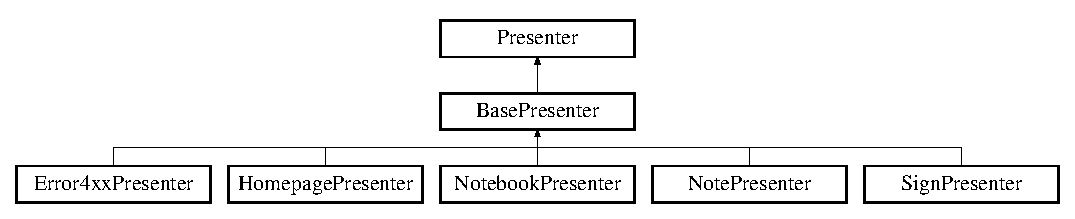
\includegraphics[height=2.488889cm]{class_app_1_1_presenters_1_1_base_presenter}
\end{center}
\end{figure}
\subsection*{Protected Member Functions}
\begin{DoxyCompactItemize}
\item 
\mbox{\hyperlink{class_app_1_1_presenters_1_1_base_presenter_ac82bc6601e7d9ed8f142734573463465}{log\+Check}} ()
\end{DoxyCompactItemize}


\subsection{Member Function Documentation}
\mbox{\Hypertarget{class_app_1_1_presenters_1_1_base_presenter_ac82bc6601e7d9ed8f142734573463465}\label{class_app_1_1_presenters_1_1_base_presenter_ac82bc6601e7d9ed8f142734573463465}} 
\index{App\+::\+Presenters\+::\+Base\+Presenter@{App\+::\+Presenters\+::\+Base\+Presenter}!log\+Check@{log\+Check}}
\index{log\+Check@{log\+Check}!App\+::\+Presenters\+::\+Base\+Presenter@{App\+::\+Presenters\+::\+Base\+Presenter}}
\subsubsection{\texorpdfstring{log\+Check()}{logCheck()}}
{\footnotesize\ttfamily log\+Check (\begin{DoxyParamCaption}{ }\end{DoxyParamCaption})\hspace{0.3cm}{\ttfamily [protected]}}

Function responsible for checking whether the user is logged in or not. 

The documentation for this class was generated from the following file\+:\begin{DoxyCompactItemize}
\item 
Base\+Presenter.\+php\end{DoxyCompactItemize}

\section{Error4xx\+Presenter Class Reference}
\label{class_app_1_1_presenters_1_1_error4xx_presenter}\index{Error4xx\+Presenter@{Error4xx\+Presenter}}
Inheritance diagram for Error4xx\+Presenter\+:\begin{figure}[H]
\begin{center}
\leavevmode
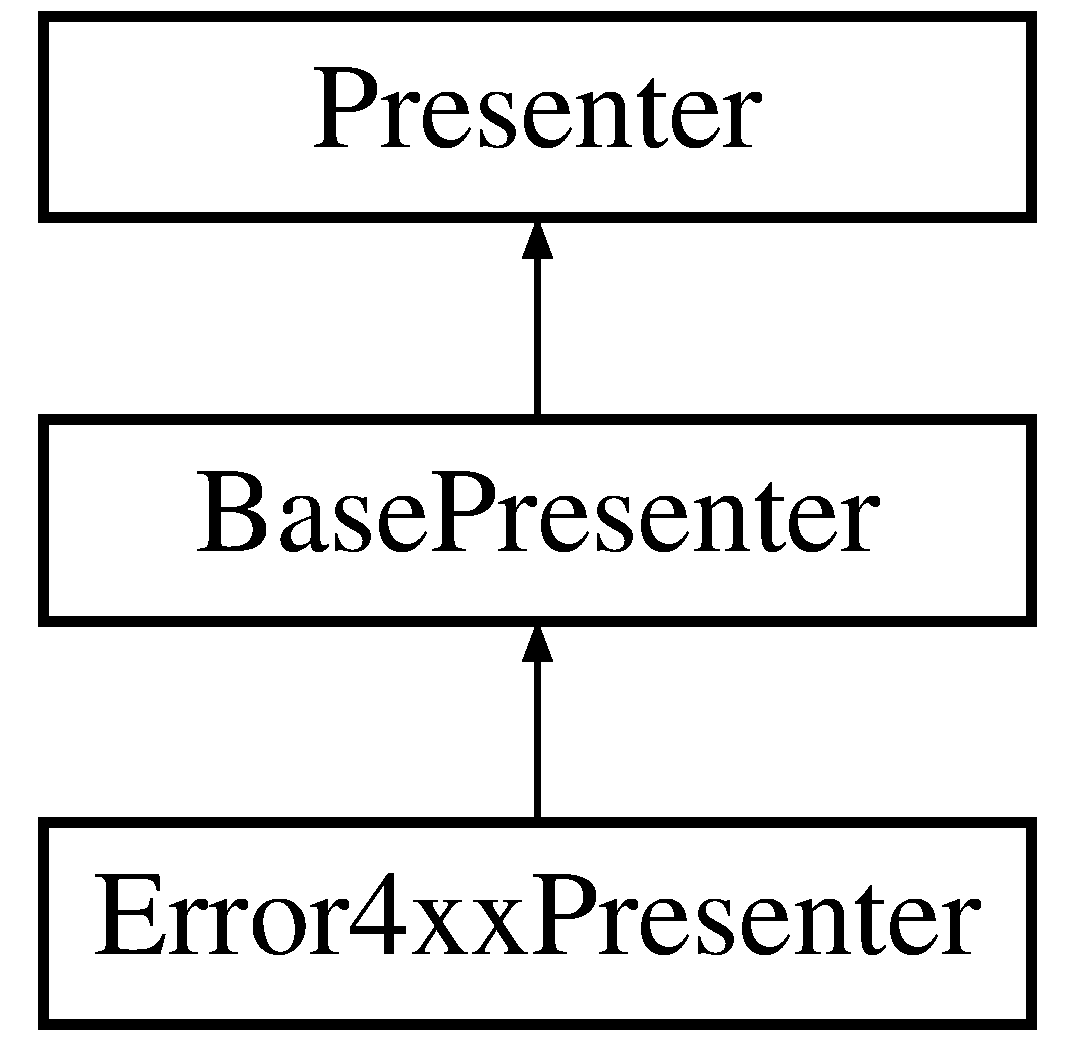
\includegraphics[height=3.000000cm]{class_app_1_1_presenters_1_1_error4xx_presenter}
\end{center}
\end{figure}
\subsection*{Public Member Functions}
\begin{DoxyCompactItemize}
\item 
\mbox{\label{class_app_1_1_presenters_1_1_error4xx_presenter_aca47505b8732177f52bb2d647eb2741c}} 
{\bfseries startup} ()
\item 
\mbox{\label{class_app_1_1_presenters_1_1_error4xx_presenter_a57df1339c0adc6203f2e02bcddc435aa}} 
{\bfseries render\+Default} (Nette\textbackslash{}\+Application\textbackslash{}\+Bad\+Request\+Exception \$exception)
\end{DoxyCompactItemize}
\subsection*{Additional Inherited Members}


The documentation for this class was generated from the following file\+:\begin{DoxyCompactItemize}
\item 
app/presenters/Error4xx\+Presenter.\+php\end{DoxyCompactItemize}

\hypertarget{class_app_1_1_presenters_1_1_error_presenter}{}\section{Error\+Presenter Class Reference}
\label{class_app_1_1_presenters_1_1_error_presenter}\index{Error\+Presenter@{Error\+Presenter}}
Inheritance diagram for Error\+Presenter\+:\begin{figure}[H]
\begin{center}
\leavevmode
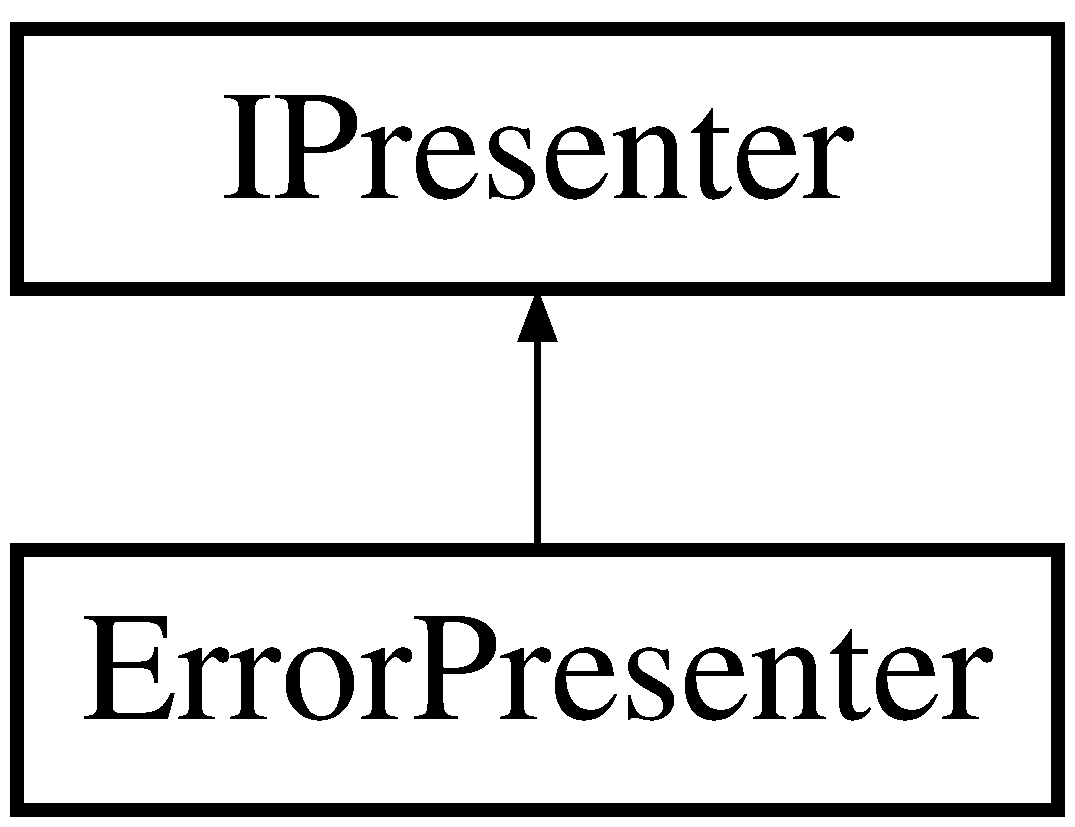
\includegraphics[height=2.000000cm]{class_app_1_1_presenters_1_1_error_presenter}
\end{center}
\end{figure}
\subsection*{Public Member Functions}
\begin{DoxyCompactItemize}
\item 
\mbox{\hyperlink{class_app_1_1_presenters_1_1_error_presenter_a47dfcedb8bbffa17106ec84907a2f101}{\+\_\+\+\_\+construct}} (I\+Logger \$logger)
\item 
\mbox{\hyperlink{class_app_1_1_presenters_1_1_error_presenter_a7d2a09004db8fd54068d96170b66654c}{run}} (Nette\textbackslash{}\+Application\textbackslash{}\+Request \$request)
\end{DoxyCompactItemize}


\subsection{Constructor \& Destructor Documentation}
\mbox{\Hypertarget{class_app_1_1_presenters_1_1_error_presenter_a47dfcedb8bbffa17106ec84907a2f101}\label{class_app_1_1_presenters_1_1_error_presenter_a47dfcedb8bbffa17106ec84907a2f101}} 
\index{App\+::\+Presenters\+::\+Error\+Presenter@{App\+::\+Presenters\+::\+Error\+Presenter}!\+\_\+\+\_\+construct@{\+\_\+\+\_\+construct}}
\index{\+\_\+\+\_\+construct@{\+\_\+\+\_\+construct}!App\+::\+Presenters\+::\+Error\+Presenter@{App\+::\+Presenters\+::\+Error\+Presenter}}
\subsubsection{\texorpdfstring{\+\_\+\+\_\+construct()}{\_\_construct()}}
{\footnotesize\ttfamily \+\_\+\+\_\+construct (\begin{DoxyParamCaption}\item[{I\+Logger}]{\$logger }\end{DoxyParamCaption})}

\mbox{\hyperlink{class_app_1_1_presenters_1_1_error_presenter}{Error\+Presenter}} constructor.


\begin{DoxyParams}[1]{Parameters}
I\+Logger & {\em \$logger} & \\
\hline
\end{DoxyParams}


\subsection{Member Function Documentation}
\mbox{\Hypertarget{class_app_1_1_presenters_1_1_error_presenter_a7d2a09004db8fd54068d96170b66654c}\label{class_app_1_1_presenters_1_1_error_presenter_a7d2a09004db8fd54068d96170b66654c}} 
\index{App\+::\+Presenters\+::\+Error\+Presenter@{App\+::\+Presenters\+::\+Error\+Presenter}!run@{run}}
\index{run@{run}!App\+::\+Presenters\+::\+Error\+Presenter@{App\+::\+Presenters\+::\+Error\+Presenter}}
\subsubsection{\texorpdfstring{run()}{run()}}
{\footnotesize\ttfamily run (\begin{DoxyParamCaption}\item[{Nette\textbackslash{}\+Application\textbackslash{}\+Request}]{\$request }\end{DoxyParamCaption})}

\begin{DoxyReturn}{Returns}
Nette 
\end{DoxyReturn}


The documentation for this class was generated from the following file\+:\begin{DoxyCompactItemize}
\item 
Error\+Presenter.\+php\end{DoxyCompactItemize}

\hypertarget{class_app_1_1_presenters_1_1_homepage_presenter}{}\section{Homepage\+Presenter Class Reference}
\label{class_app_1_1_presenters_1_1_homepage_presenter}\index{Homepage\+Presenter@{Homepage\+Presenter}}
Inheritance diagram for Homepage\+Presenter\+:\begin{figure}[H]
\begin{center}
\leavevmode
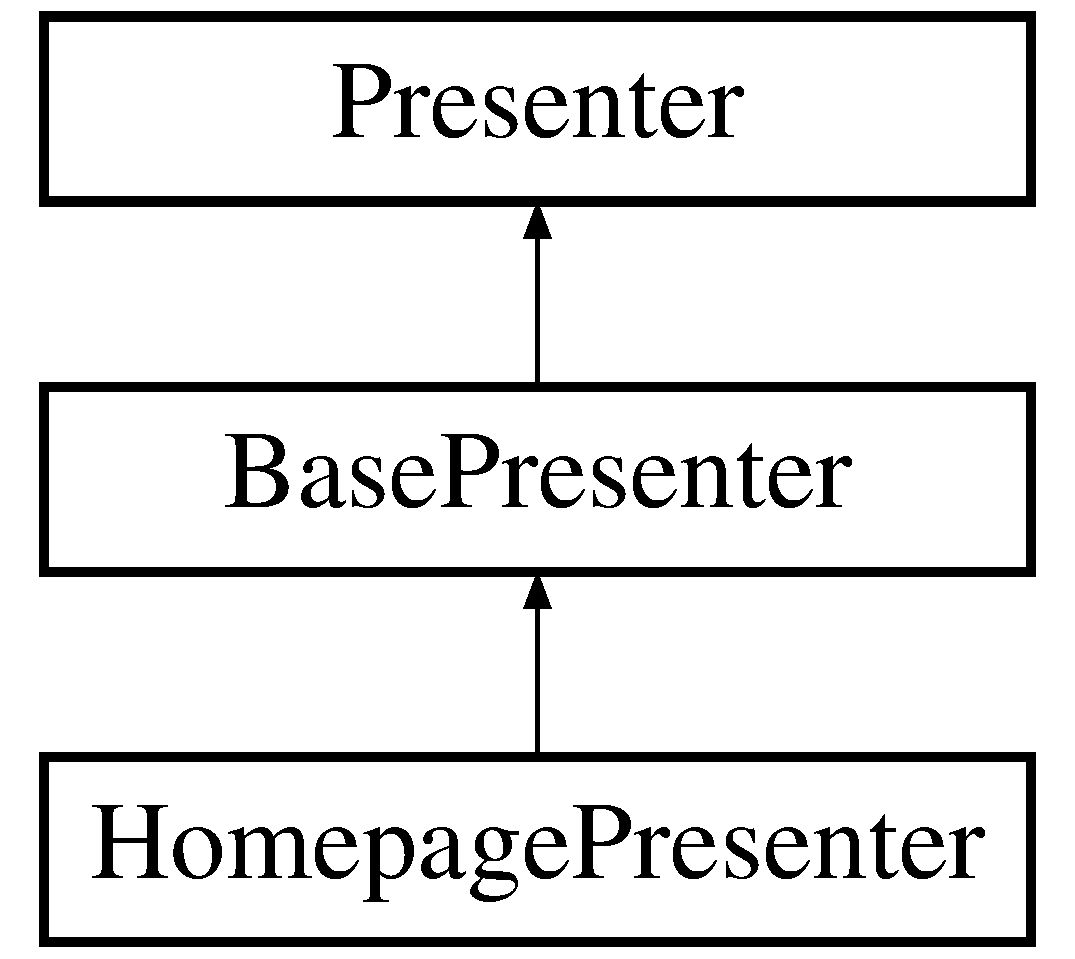
\includegraphics[height=3.000000cm]{class_app_1_1_presenters_1_1_homepage_presenter}
\end{center}
\end{figure}
\subsection*{Public Member Functions}
\begin{DoxyCompactItemize}
\item 
\mbox{\hyperlink{class_app_1_1_presenters_1_1_homepage_presenter_abf10af0e00d40379ce44c79183832689}{\+\_\+\+\_\+construct}} (Notebook\+Manager \$notebook\+Manager, Note\+Manager \$note\+Manager)
\item 
\mbox{\hyperlink{class_app_1_1_presenters_1_1_homepage_presenter_a1090bf761e1e8e9243cb3062c11600db}{action\+Default}} (\$page=1)
\item 
\mbox{\hyperlink{class_app_1_1_presenters_1_1_homepage_presenter_a7824b03de268f5968857a8ea1b23abe0}{render\+Default}} (\$page=1)
\item 
\mbox{\hyperlink{class_app_1_1_presenters_1_1_homepage_presenter_a40f94e2f3bc673ae3f7190f002fef637}{create\+Component\+Quick\+Note\+Form}} ()
\item 
\mbox{\hyperlink{class_app_1_1_presenters_1_1_homepage_presenter_a6bff9f0e53d83bc12b862f35d28913b6}{create\+Component\+Notebook\+Add\+Form}} ()
\item 
\mbox{\hyperlink{class_app_1_1_presenters_1_1_homepage_presenter_ae4cce48b067df705c3a2c984fa74f3a9}{quick\+Note\+Form\+Succeeded}} (\$form, \$values)
\item 
\mbox{\hyperlink{class_app_1_1_presenters_1_1_homepage_presenter_a5579f6a3db49483e429a74ba2b638b43}{notebook\+Add\+Form\+Succeeded}} (\$form, \$values)
\end{DoxyCompactItemize}
\subsection*{Additional Inherited Members}


\subsection{Constructor \& Destructor Documentation}
\mbox{\Hypertarget{class_app_1_1_presenters_1_1_homepage_presenter_abf10af0e00d40379ce44c79183832689}\label{class_app_1_1_presenters_1_1_homepage_presenter_abf10af0e00d40379ce44c79183832689}} 
\index{App\+::\+Presenters\+::\+Homepage\+Presenter@{App\+::\+Presenters\+::\+Homepage\+Presenter}!\+\_\+\+\_\+construct@{\+\_\+\+\_\+construct}}
\index{\+\_\+\+\_\+construct@{\+\_\+\+\_\+construct}!App\+::\+Presenters\+::\+Homepage\+Presenter@{App\+::\+Presenters\+::\+Homepage\+Presenter}}
\subsubsection{\texorpdfstring{\+\_\+\+\_\+construct()}{\_\_construct()}}
{\footnotesize\ttfamily \+\_\+\+\_\+construct (\begin{DoxyParamCaption}\item[{Notebook\+Manager}]{\$notebook\+Manager,  }\item[{Note\+Manager}]{\$note\+Manager }\end{DoxyParamCaption})}

\mbox{\hyperlink{class_app_1_1_presenters_1_1_homepage_presenter}{Homepage\+Presenter}} constructor.


\begin{DoxyParams}[1]{Parameters}
Notebook\+Manager & {\em \$notebook\+Manager} & \\
\hline
Note\+Manager & {\em \$note\+Manager} & \\
\hline
\end{DoxyParams}


\subsection{Member Function Documentation}
\mbox{\Hypertarget{class_app_1_1_presenters_1_1_homepage_presenter_a1090bf761e1e8e9243cb3062c11600db}\label{class_app_1_1_presenters_1_1_homepage_presenter_a1090bf761e1e8e9243cb3062c11600db}} 
\index{App\+::\+Presenters\+::\+Homepage\+Presenter@{App\+::\+Presenters\+::\+Homepage\+Presenter}!action\+Default@{action\+Default}}
\index{action\+Default@{action\+Default}!App\+::\+Presenters\+::\+Homepage\+Presenter@{App\+::\+Presenters\+::\+Homepage\+Presenter}}
\subsubsection{\texorpdfstring{action\+Default()}{actionDefault()}}
{\footnotesize\ttfamily action\+Default (\begin{DoxyParamCaption}\item[{}]{\$page = {\ttfamily 1} }\end{DoxyParamCaption})}

Default action -\/ just checks login.


\begin{DoxyParams}[1]{Parameters}
int & {\em \$page} & Paginator page \\
\hline
\end{DoxyParams}
\mbox{\Hypertarget{class_app_1_1_presenters_1_1_homepage_presenter_a6bff9f0e53d83bc12b862f35d28913b6}\label{class_app_1_1_presenters_1_1_homepage_presenter_a6bff9f0e53d83bc12b862f35d28913b6}} 
\index{App\+::\+Presenters\+::\+Homepage\+Presenter@{App\+::\+Presenters\+::\+Homepage\+Presenter}!create\+Component\+Notebook\+Add\+Form@{create\+Component\+Notebook\+Add\+Form}}
\index{create\+Component\+Notebook\+Add\+Form@{create\+Component\+Notebook\+Add\+Form}!App\+::\+Presenters\+::\+Homepage\+Presenter@{App\+::\+Presenters\+::\+Homepage\+Presenter}}
\subsubsection{\texorpdfstring{create\+Component\+Notebook\+Add\+Form()}{createComponentNotebookAddForm()}}
{\footnotesize\ttfamily create\+Component\+Notebook\+Add\+Form (\begin{DoxyParamCaption}{ }\end{DoxyParamCaption})}

Creates notebook\+Add form.

\begin{DoxyReturn}{Returns}
Form Notebook\+Add form with headline and description 
\end{DoxyReturn}
\mbox{\Hypertarget{class_app_1_1_presenters_1_1_homepage_presenter_a40f94e2f3bc673ae3f7190f002fef637}\label{class_app_1_1_presenters_1_1_homepage_presenter_a40f94e2f3bc673ae3f7190f002fef637}} 
\index{App\+::\+Presenters\+::\+Homepage\+Presenter@{App\+::\+Presenters\+::\+Homepage\+Presenter}!create\+Component\+Quick\+Note\+Form@{create\+Component\+Quick\+Note\+Form}}
\index{create\+Component\+Quick\+Note\+Form@{create\+Component\+Quick\+Note\+Form}!App\+::\+Presenters\+::\+Homepage\+Presenter@{App\+::\+Presenters\+::\+Homepage\+Presenter}}
\subsubsection{\texorpdfstring{create\+Component\+Quick\+Note\+Form()}{createComponentQuickNoteForm()}}
{\footnotesize\ttfamily create\+Component\+Quick\+Note\+Form (\begin{DoxyParamCaption}{ }\end{DoxyParamCaption})}

Creates quick\+Notes form.

\begin{DoxyReturn}{Returns}
Form Quick\+Note form with headline and content 
\end{DoxyReturn}
\mbox{\Hypertarget{class_app_1_1_presenters_1_1_homepage_presenter_a5579f6a3db49483e429a74ba2b638b43}\label{class_app_1_1_presenters_1_1_homepage_presenter_a5579f6a3db49483e429a74ba2b638b43}} 
\index{App\+::\+Presenters\+::\+Homepage\+Presenter@{App\+::\+Presenters\+::\+Homepage\+Presenter}!notebook\+Add\+Form\+Succeeded@{notebook\+Add\+Form\+Succeeded}}
\index{notebook\+Add\+Form\+Succeeded@{notebook\+Add\+Form\+Succeeded}!App\+::\+Presenters\+::\+Homepage\+Presenter@{App\+::\+Presenters\+::\+Homepage\+Presenter}}
\subsubsection{\texorpdfstring{notebook\+Add\+Form\+Succeeded()}{notebookAddFormSucceeded()}}
{\footnotesize\ttfamily notebook\+Add\+Form\+Succeeded (\begin{DoxyParamCaption}\item[{}]{\$form,  }\item[{}]{\$values }\end{DoxyParamCaption})}

Function called after successful notebook\+Add\+Form submit. It is responsible for adding notebook for user.


\begin{DoxyParams}{Parameters}
{\em \$form} & Form Notebook\+Add form \\
\hline
{\em \$values} & array Array of values returned by Notebook\+Add form \\
\hline
\end{DoxyParams}
\mbox{\Hypertarget{class_app_1_1_presenters_1_1_homepage_presenter_ae4cce48b067df705c3a2c984fa74f3a9}\label{class_app_1_1_presenters_1_1_homepage_presenter_ae4cce48b067df705c3a2c984fa74f3a9}} 
\index{App\+::\+Presenters\+::\+Homepage\+Presenter@{App\+::\+Presenters\+::\+Homepage\+Presenter}!quick\+Note\+Form\+Succeeded@{quick\+Note\+Form\+Succeeded}}
\index{quick\+Note\+Form\+Succeeded@{quick\+Note\+Form\+Succeeded}!App\+::\+Presenters\+::\+Homepage\+Presenter@{App\+::\+Presenters\+::\+Homepage\+Presenter}}
\subsubsection{\texorpdfstring{quick\+Note\+Form\+Succeeded()}{quickNoteFormSucceeded()}}
{\footnotesize\ttfamily quick\+Note\+Form\+Succeeded (\begin{DoxyParamCaption}\item[{}]{\$form,  }\item[{}]{\$values }\end{DoxyParamCaption})}

Function called after successful quick\+Note\+Form submit. It is responsible for check of Quick\+Notes Notebook existance and int\textquotesingle{}s creation when necessary and adding the quick note.


\begin{DoxyParams}{Parameters}
{\em \$form} & Form Quick\+Note form \\
\hline
{\em \$values} & array Array of values returned by Quick\+Note form \\
\hline
\end{DoxyParams}
\mbox{\Hypertarget{class_app_1_1_presenters_1_1_homepage_presenter_a7824b03de268f5968857a8ea1b23abe0}\label{class_app_1_1_presenters_1_1_homepage_presenter_a7824b03de268f5968857a8ea1b23abe0}} 
\index{App\+::\+Presenters\+::\+Homepage\+Presenter@{App\+::\+Presenters\+::\+Homepage\+Presenter}!render\+Default@{render\+Default}}
\index{render\+Default@{render\+Default}!App\+::\+Presenters\+::\+Homepage\+Presenter@{App\+::\+Presenters\+::\+Homepage\+Presenter}}
\subsubsection{\texorpdfstring{render\+Default()}{renderDefault()}}
{\footnotesize\ttfamily render\+Default (\begin{DoxyParamCaption}\item[{}]{\$page = {\ttfamily 1} }\end{DoxyParamCaption})}

Renders default template -\/ list of all user notebooks.


\begin{DoxyParams}[1]{Parameters}
int & {\em \$page} & Paginator page \\
\hline
\end{DoxyParams}


The documentation for this class was generated from the following file\+:\begin{DoxyCompactItemize}
\item 
Homepage\+Presenter.\+php\end{DoxyCompactItemize}

\section{Notebook\+Presenter Class Reference}
\label{class_app_1_1_presenters_1_1_notebook_presenter}\index{Notebook\+Presenter@{Notebook\+Presenter}}
Inheritance diagram for Notebook\+Presenter\+:\begin{figure}[H]
\begin{center}
\leavevmode
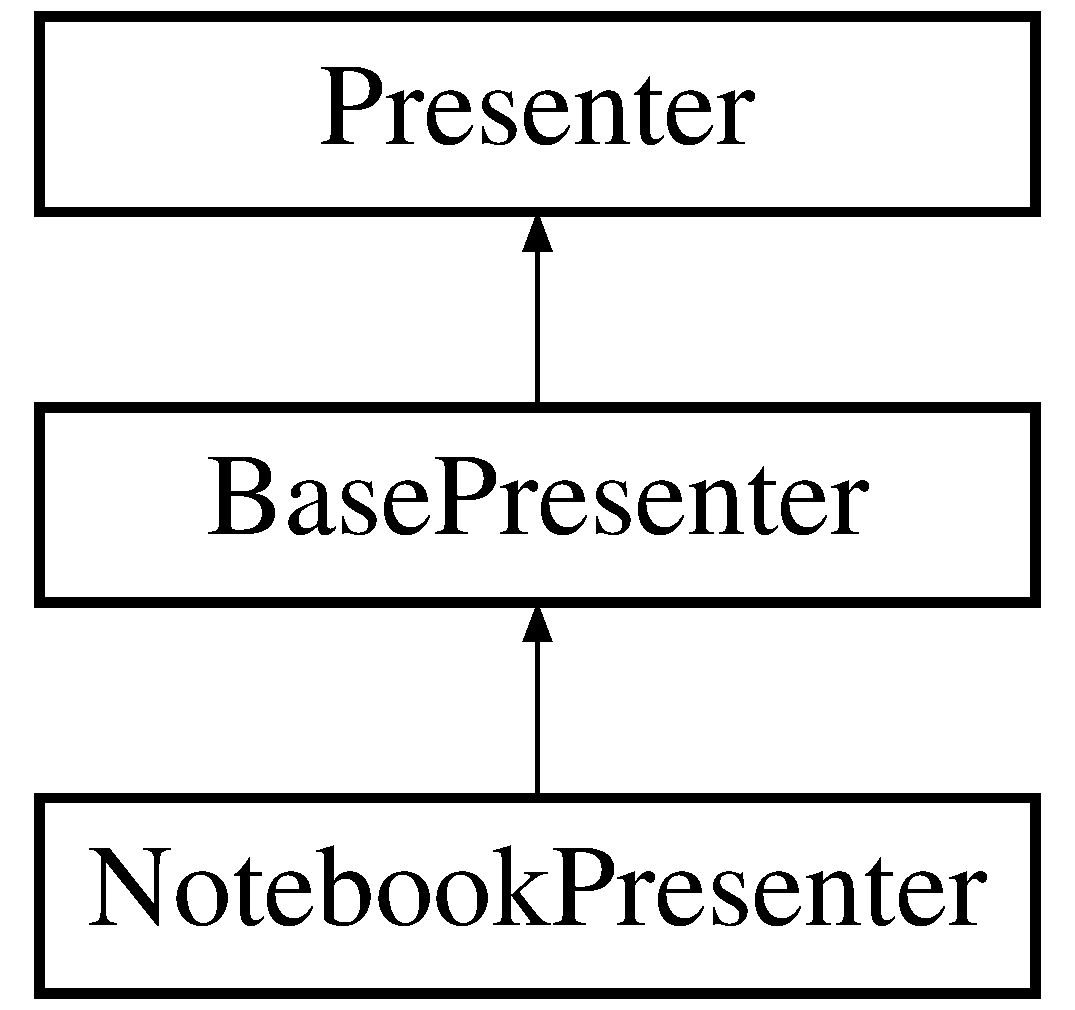
\includegraphics[height=3.000000cm]{class_app_1_1_presenters_1_1_notebook_presenter}
\end{center}
\end{figure}
\subsection*{Public Member Functions}
\begin{DoxyCompactItemize}
\item 
\textbf{ \+\_\+\+\_\+construct} (\textbf{ Notebook\+Manager} \$notebook\+Manager, \textbf{ Note\+Manager} \$note\+Manager)
\item 
\textbf{ action\+Default} (\$id, \$page=1)
\item 
\textbf{ render\+Default} (\$id, \$page=1)
\item 
\textbf{ action\+Remove} (\$id)
\item 
\textbf{ create\+Component\+Note\+Add\+Form} ()
\item 
\textbf{ note\+Add\+Form\+Succeeded} (\$form, \$values)
\end{DoxyCompactItemize}
\subsection*{Additional Inherited Members}


\subsection{Constructor \& Destructor Documentation}
\mbox{\label{class_app_1_1_presenters_1_1_notebook_presenter_abf10af0e00d40379ce44c79183832689}} 
\index{App\+::\+Presenters\+::\+Notebook\+Presenter@{App\+::\+Presenters\+::\+Notebook\+Presenter}!\+\_\+\+\_\+construct@{\+\_\+\+\_\+construct}}
\index{\+\_\+\+\_\+construct@{\+\_\+\+\_\+construct}!App\+::\+Presenters\+::\+Notebook\+Presenter@{App\+::\+Presenters\+::\+Notebook\+Presenter}}
\subsubsection{\+\_\+\+\_\+construct()}
{\footnotesize\ttfamily \+\_\+\+\_\+construct (\begin{DoxyParamCaption}\item[{\textbf{ Notebook\+Manager}}]{\$notebook\+Manager,  }\item[{\textbf{ Note\+Manager}}]{\$note\+Manager }\end{DoxyParamCaption})}

\doxyref{Notebook\+Presenter}{p.}{class_app_1_1_presenters_1_1_notebook_presenter} constructor.


\begin{DoxyParams}[1]{Parameters}
Notebook\+Manager & {\em \$notebook\+Manager} & \doxyref{Model}{p.}{namespace_app_1_1_model} working with notebooks table \\
\hline
Note\+Manager & {\em \$note\+Manager} & \doxyref{Model}{p.}{namespace_app_1_1_model} working with notes table \\
\hline
\end{DoxyParams}


\subsection{Member Function Documentation}
\mbox{\label{class_app_1_1_presenters_1_1_notebook_presenter_a3b0019dbdf5a7e4547275d3be02e1f7d}} 
\index{App\+::\+Presenters\+::\+Notebook\+Presenter@{App\+::\+Presenters\+::\+Notebook\+Presenter}!action\+Default@{action\+Default}}
\index{action\+Default@{action\+Default}!App\+::\+Presenters\+::\+Notebook\+Presenter@{App\+::\+Presenters\+::\+Notebook\+Presenter}}
\subsubsection{action\+Default()}
{\footnotesize\ttfamily action\+Default (\begin{DoxyParamCaption}\item[{}]{\$id,  }\item[{}]{\$page = {\ttfamily 1} }\end{DoxyParamCaption})}

Performs actions before rendering the notebook view.


\begin{DoxyParams}[1]{Parameters}
int & {\em \$id} & ID of notebook to be displayed \\
\hline
int & {\em \$page} & Paginator page \\
\hline
\end{DoxyParams}
\mbox{\label{class_app_1_1_presenters_1_1_notebook_presenter_ab7e4d6093e671c38971e19e7a45f322b}} 
\index{App\+::\+Presenters\+::\+Notebook\+Presenter@{App\+::\+Presenters\+::\+Notebook\+Presenter}!action\+Remove@{action\+Remove}}
\index{action\+Remove@{action\+Remove}!App\+::\+Presenters\+::\+Notebook\+Presenter@{App\+::\+Presenters\+::\+Notebook\+Presenter}}
\subsubsection{action\+Remove()}
{\footnotesize\ttfamily action\+Remove (\begin{DoxyParamCaption}\item[{}]{\$id }\end{DoxyParamCaption})}

Function responsible for removing note. It checks ownership and so on.


\begin{DoxyParams}[1]{Parameters}
int & {\em \$id} & ID of note to be removed \\
\hline
\end{DoxyParams}
\mbox{\label{class_app_1_1_presenters_1_1_notebook_presenter_a43f32165e9c04e87af5d78509076ea53}} 
\index{App\+::\+Presenters\+::\+Notebook\+Presenter@{App\+::\+Presenters\+::\+Notebook\+Presenter}!create\+Component\+Note\+Add\+Form@{create\+Component\+Note\+Add\+Form}}
\index{create\+Component\+Note\+Add\+Form@{create\+Component\+Note\+Add\+Form}!App\+::\+Presenters\+::\+Notebook\+Presenter@{App\+::\+Presenters\+::\+Notebook\+Presenter}}
\subsubsection{create\+Component\+Note\+Add\+Form()}
{\footnotesize\ttfamily create\+Component\+Note\+Add\+Form (\begin{DoxyParamCaption}{ }\end{DoxyParamCaption})}

Function creating the Note\+Add form

\begin{DoxyReturn}{Returns}
Form Note\+Add form with hiddne notebook\+ID and headline + content inputs 
\end{DoxyReturn}
\mbox{\label{class_app_1_1_presenters_1_1_notebook_presenter_af4e4ada78cf634f26140f658dc710c06}} 
\index{App\+::\+Presenters\+::\+Notebook\+Presenter@{App\+::\+Presenters\+::\+Notebook\+Presenter}!note\+Add\+Form\+Succeeded@{note\+Add\+Form\+Succeeded}}
\index{note\+Add\+Form\+Succeeded@{note\+Add\+Form\+Succeeded}!App\+::\+Presenters\+::\+Notebook\+Presenter@{App\+::\+Presenters\+::\+Notebook\+Presenter}}
\subsubsection{note\+Add\+Form\+Succeeded()}
{\footnotesize\ttfamily note\+Add\+Form\+Succeeded (\begin{DoxyParamCaption}\item[{}]{\$form,  }\item[{}]{\$values }\end{DoxyParamCaption})}

Function called after successful note\+Add submit. It is resposbile for note addition and notifying the user.


\begin{DoxyParams}{Parameters}
{\em \$form} & \\
\hline
{\em \$values} & \\
\hline
\end{DoxyParams}
\mbox{\label{class_app_1_1_presenters_1_1_notebook_presenter_a0abea8519a466f30d4fe2a7b9e2872f8}} 
\index{App\+::\+Presenters\+::\+Notebook\+Presenter@{App\+::\+Presenters\+::\+Notebook\+Presenter}!render\+Default@{render\+Default}}
\index{render\+Default@{render\+Default}!App\+::\+Presenters\+::\+Notebook\+Presenter@{App\+::\+Presenters\+::\+Notebook\+Presenter}}
\subsubsection{render\+Default()}
{\footnotesize\ttfamily render\+Default (\begin{DoxyParamCaption}\item[{}]{\$id,  }\item[{}]{\$page = {\ttfamily 1} }\end{DoxyParamCaption})}

Renders default notebook page based on


\begin{DoxyParams}[1]{Parameters}
int & {\em \$id} & ID of notebook to be displayed \\
\hline
int & {\em \$page} & Paginator page \\
\hline
\end{DoxyParams}


The documentation for this class was generated from the following file\+:\begin{DoxyCompactItemize}
\item 
app/presenters/Notebook\+Presenter.\+php\end{DoxyCompactItemize}

\hypertarget{class_app_1_1_presenters_1_1_note_presenter}{}\section{Note\+Presenter Class Reference}
\label{class_app_1_1_presenters_1_1_note_presenter}\index{Note\+Presenter@{Note\+Presenter}}
Inheritance diagram for Note\+Presenter\+:\begin{figure}[H]
\begin{center}
\leavevmode
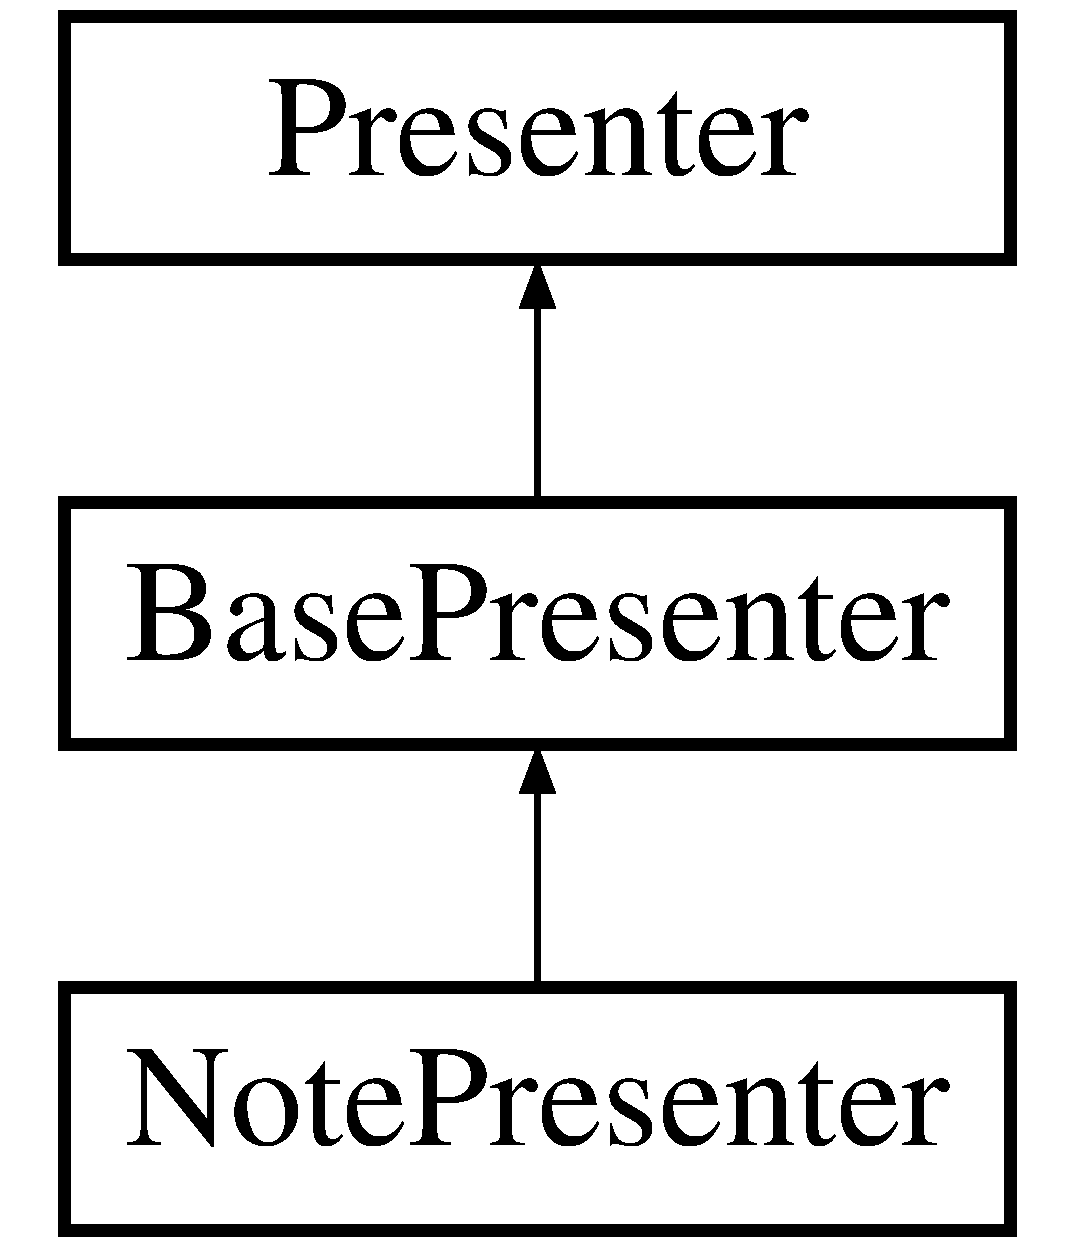
\includegraphics[height=3.000000cm]{class_app_1_1_presenters_1_1_note_presenter}
\end{center}
\end{figure}
\subsection*{Public Member Functions}
\begin{DoxyCompactItemize}
\item 
\mbox{\hyperlink{class_app_1_1_presenters_1_1_note_presenter_abf10af0e00d40379ce44c79183832689}{\+\_\+\+\_\+construct}} (Notebook\+Manager \$notebook\+Manager, Note\+Manager \$note\+Manager)
\item 
\mbox{\hyperlink{class_app_1_1_presenters_1_1_note_presenter_abc9fade9634c03fc324b4559fbe2abfb}{action\+Default}} (\$id)
\item 
\mbox{\hyperlink{class_app_1_1_presenters_1_1_note_presenter_ac57e2ee064c6a891f41051ef6e116c1f}{render\+Default}} (\$id)
\item 
\mbox{\hyperlink{class_app_1_1_presenters_1_1_note_presenter_ab7e4d6093e671c38971e19e7a45f322b}{action\+Remove}} (\$id)
\item 
\mbox{\hyperlink{class_app_1_1_presenters_1_1_note_presenter_adbe06f4aac8adda69c1cf4cefcc9c58d}{create\+Component\+Note\+Edit\+Form}} ()
\item 
\mbox{\hyperlink{class_app_1_1_presenters_1_1_note_presenter_a31fc3d689c7087bb9650b232ce35cca3}{note\+Edit\+Form\+Succeeded}} (\$form, \$values)
\end{DoxyCompactItemize}
\subsection*{Additional Inherited Members}


\subsection{Constructor \& Destructor Documentation}
\mbox{\Hypertarget{class_app_1_1_presenters_1_1_note_presenter_abf10af0e00d40379ce44c79183832689}\label{class_app_1_1_presenters_1_1_note_presenter_abf10af0e00d40379ce44c79183832689}} 
\index{App\+::\+Presenters\+::\+Note\+Presenter@{App\+::\+Presenters\+::\+Note\+Presenter}!\+\_\+\+\_\+construct@{\+\_\+\+\_\+construct}}
\index{\+\_\+\+\_\+construct@{\+\_\+\+\_\+construct}!App\+::\+Presenters\+::\+Note\+Presenter@{App\+::\+Presenters\+::\+Note\+Presenter}}
\subsubsection{\texorpdfstring{\+\_\+\+\_\+construct()}{\_\_construct()}}
{\footnotesize\ttfamily \+\_\+\+\_\+construct (\begin{DoxyParamCaption}\item[{Notebook\+Manager}]{\$notebook\+Manager,  }\item[{Note\+Manager}]{\$note\+Manager }\end{DoxyParamCaption})}

\mbox{\hyperlink{class_app_1_1_presenters_1_1_note_presenter}{Note\+Presenter}} constructor.


\begin{DoxyParams}[1]{Parameters}
Notebook\+Manager & {\em \$notebook\+Manager} & Model working with notebooks table \\
\hline
Note\+Manager & {\em \$note\+Manager} & Model working with notes table \\
\hline
\end{DoxyParams}


\subsection{Member Function Documentation}
\mbox{\Hypertarget{class_app_1_1_presenters_1_1_note_presenter_abc9fade9634c03fc324b4559fbe2abfb}\label{class_app_1_1_presenters_1_1_note_presenter_abc9fade9634c03fc324b4559fbe2abfb}} 
\index{App\+::\+Presenters\+::\+Note\+Presenter@{App\+::\+Presenters\+::\+Note\+Presenter}!action\+Default@{action\+Default}}
\index{action\+Default@{action\+Default}!App\+::\+Presenters\+::\+Note\+Presenter@{App\+::\+Presenters\+::\+Note\+Presenter}}
\subsubsection{\texorpdfstring{action\+Default()}{actionDefault()}}
{\footnotesize\ttfamily action\+Default (\begin{DoxyParamCaption}\item[{}]{\$id }\end{DoxyParamCaption})}

Performs actions before rendering the note view.


\begin{DoxyParams}{Parameters}
{\em \$id} & int ID of note to be displayed \\
\hline
\end{DoxyParams}
\mbox{\Hypertarget{class_app_1_1_presenters_1_1_note_presenter_ab7e4d6093e671c38971e19e7a45f322b}\label{class_app_1_1_presenters_1_1_note_presenter_ab7e4d6093e671c38971e19e7a45f322b}} 
\index{App\+::\+Presenters\+::\+Note\+Presenter@{App\+::\+Presenters\+::\+Note\+Presenter}!action\+Remove@{action\+Remove}}
\index{action\+Remove@{action\+Remove}!App\+::\+Presenters\+::\+Note\+Presenter@{App\+::\+Presenters\+::\+Note\+Presenter}}
\subsubsection{\texorpdfstring{action\+Remove()}{actionRemove()}}
{\footnotesize\ttfamily action\+Remove (\begin{DoxyParamCaption}\item[{}]{\$id }\end{DoxyParamCaption})}

Action responsible for removing the note from database.


\begin{DoxyParams}{Parameters}
{\em \$id} & int ID of note to be removed \\
\hline
\end{DoxyParams}
\mbox{\Hypertarget{class_app_1_1_presenters_1_1_note_presenter_adbe06f4aac8adda69c1cf4cefcc9c58d}\label{class_app_1_1_presenters_1_1_note_presenter_adbe06f4aac8adda69c1cf4cefcc9c58d}} 
\index{App\+::\+Presenters\+::\+Note\+Presenter@{App\+::\+Presenters\+::\+Note\+Presenter}!create\+Component\+Note\+Edit\+Form@{create\+Component\+Note\+Edit\+Form}}
\index{create\+Component\+Note\+Edit\+Form@{create\+Component\+Note\+Edit\+Form}!App\+::\+Presenters\+::\+Note\+Presenter@{App\+::\+Presenters\+::\+Note\+Presenter}}
\subsubsection{\texorpdfstring{create\+Component\+Note\+Edit\+Form()}{createComponentNoteEditForm()}}
{\footnotesize\ttfamily create\+Component\+Note\+Edit\+Form (\begin{DoxyParamCaption}{ }\end{DoxyParamCaption})}

Function creating the Note\+Edit form.

\begin{DoxyReturn}{Returns}
Form Note\+Edit form with hidden note\+ID, headline and content of note 
\end{DoxyReturn}
\mbox{\Hypertarget{class_app_1_1_presenters_1_1_note_presenter_a31fc3d689c7087bb9650b232ce35cca3}\label{class_app_1_1_presenters_1_1_note_presenter_a31fc3d689c7087bb9650b232ce35cca3}} 
\index{App\+::\+Presenters\+::\+Note\+Presenter@{App\+::\+Presenters\+::\+Note\+Presenter}!note\+Edit\+Form\+Succeeded@{note\+Edit\+Form\+Succeeded}}
\index{note\+Edit\+Form\+Succeeded@{note\+Edit\+Form\+Succeeded}!App\+::\+Presenters\+::\+Note\+Presenter@{App\+::\+Presenters\+::\+Note\+Presenter}}
\subsubsection{\texorpdfstring{note\+Edit\+Form\+Succeeded()}{noteEditFormSucceeded()}}
{\footnotesize\ttfamily note\+Edit\+Form\+Succeeded (\begin{DoxyParamCaption}\item[{}]{\$form,  }\item[{}]{\$values }\end{DoxyParamCaption})}

Function called after successful note\+Edit submit. It is responsible for performing changes in the database.


\begin{DoxyParams}{Parameters}
{\em \$form} & \\
\hline
{\em \$values} & \\
\hline
\end{DoxyParams}
\mbox{\Hypertarget{class_app_1_1_presenters_1_1_note_presenter_ac57e2ee064c6a891f41051ef6e116c1f}\label{class_app_1_1_presenters_1_1_note_presenter_ac57e2ee064c6a891f41051ef6e116c1f}} 
\index{App\+::\+Presenters\+::\+Note\+Presenter@{App\+::\+Presenters\+::\+Note\+Presenter}!render\+Default@{render\+Default}}
\index{render\+Default@{render\+Default}!App\+::\+Presenters\+::\+Note\+Presenter@{App\+::\+Presenters\+::\+Note\+Presenter}}
\subsubsection{\texorpdfstring{render\+Default()}{renderDefault()}}
{\footnotesize\ttfamily render\+Default (\begin{DoxyParamCaption}\item[{}]{\$id }\end{DoxyParamCaption})}

Renders note view with corresponding note.


\begin{DoxyParams}{Parameters}
{\em \$id} & int ID of note to be displayed \\
\hline
\end{DoxyParams}


The documentation for this class was generated from the following file\+:\begin{DoxyCompactItemize}
\item 
Note\+Presenter.\+php\end{DoxyCompactItemize}

\section{Sign\+Presenter Class Reference}
\label{class_app_1_1_presenters_1_1_sign_presenter}\index{Sign\+Presenter@{Sign\+Presenter}}
Inheritance diagram for Sign\+Presenter\+:\begin{figure}[H]
\begin{center}
\leavevmode
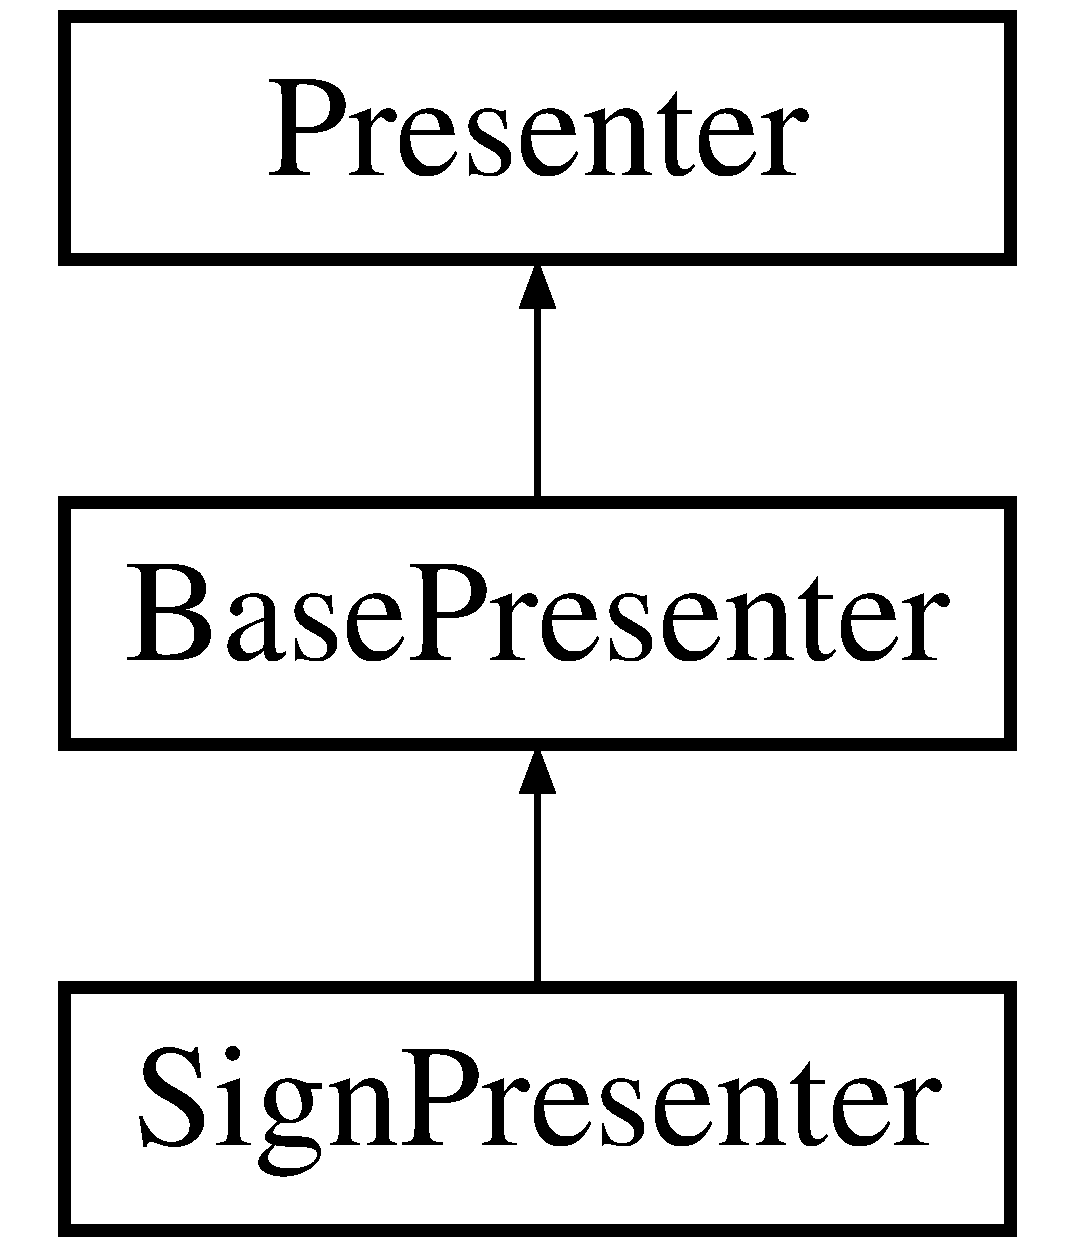
\includegraphics[height=3.000000cm]{class_app_1_1_presenters_1_1_sign_presenter}
\end{center}
\end{figure}
\subsection*{Public Member Functions}
\begin{DoxyCompactItemize}
\item 
\textbf{ \+\_\+\+\_\+construct} (\textbf{ User\+Manager} \$user\+Manager)
\item 
\textbf{ action\+Default} ()
\item 
\mbox{\label{class_app_1_1_presenters_1_1_sign_presenter_aa330fd9f860dd2ea8be435eb69e706bb}} 
{\bfseries action\+In} ()
\item 
\mbox{\label{class_app_1_1_presenters_1_1_sign_presenter_a82c9b4a056d9e439f41b5e3b9bd3b286}} 
{\bfseries action\+Up} ()
\item 
\textbf{ action\+Out} ()
\item 
\textbf{ create\+Component\+Sign\+In\+Form} ()
\item 
\textbf{ create\+Component\+Sign\+Up\+Form} ()
\item 
\textbf{ sign\+In\+Form\+Succeeded} (\$form, \$values)
\item 
\textbf{ sign\+Up\+Form\+Succeeded} (\$form, \$values)
\item 
\textbf{ handle\+Username\+Exists} (\$username)
\end{DoxyCompactItemize}
\subsection*{Additional Inherited Members}


\subsection{Constructor \& Destructor Documentation}
\mbox{\label{class_app_1_1_presenters_1_1_sign_presenter_a29d4b5fe645c2cef5f995a35d823029f}} 
\index{App\+::\+Presenters\+::\+Sign\+Presenter@{App\+::\+Presenters\+::\+Sign\+Presenter}!\+\_\+\+\_\+construct@{\+\_\+\+\_\+construct}}
\index{\+\_\+\+\_\+construct@{\+\_\+\+\_\+construct}!App\+::\+Presenters\+::\+Sign\+Presenter@{App\+::\+Presenters\+::\+Sign\+Presenter}}
\subsubsection{\+\_\+\+\_\+construct()}
{\footnotesize\ttfamily \+\_\+\+\_\+construct (\begin{DoxyParamCaption}\item[{\textbf{ User\+Manager}}]{\$user\+Manager }\end{DoxyParamCaption})}

\doxyref{Sign\+Presenter}{p.}{class_app_1_1_presenters_1_1_sign_presenter} constructor.


\begin{DoxyParams}[1]{Parameters}
User\+Manager & {\em \$user\+Manager} & \doxyref{Model}{p.}{namespace_app_1_1_model} working with users table \\
\hline
\end{DoxyParams}


\subsection{Member Function Documentation}
\mbox{\label{class_app_1_1_presenters_1_1_sign_presenter_ab3af58fdd7adf8de36403909fa255979}} 
\index{App\+::\+Presenters\+::\+Sign\+Presenter@{App\+::\+Presenters\+::\+Sign\+Presenter}!action\+Default@{action\+Default}}
\index{action\+Default@{action\+Default}!App\+::\+Presenters\+::\+Sign\+Presenter@{App\+::\+Presenters\+::\+Sign\+Presenter}}
\subsubsection{action\+Default()}
{\footnotesize\ttfamily action\+Default (\begin{DoxyParamCaption}{ }\end{DoxyParamCaption})}

Default sign function -\/ determines where to redirect user. \mbox{\label{class_app_1_1_presenters_1_1_sign_presenter_aa8143a70f2cd43780e9a2ec146b6b7c9}} 
\index{App\+::\+Presenters\+::\+Sign\+Presenter@{App\+::\+Presenters\+::\+Sign\+Presenter}!action\+Out@{action\+Out}}
\index{action\+Out@{action\+Out}!App\+::\+Presenters\+::\+Sign\+Presenter@{App\+::\+Presenters\+::\+Sign\+Presenter}}
\subsubsection{action\+Out()}
{\footnotesize\ttfamily action\+Out (\begin{DoxyParamCaption}{ }\end{DoxyParamCaption})}

Function responsible for signing out the user. \mbox{\label{class_app_1_1_presenters_1_1_sign_presenter_a3c4ccf80318992a3c1ec5e30784d1b14}} 
\index{App\+::\+Presenters\+::\+Sign\+Presenter@{App\+::\+Presenters\+::\+Sign\+Presenter}!create\+Component\+Sign\+In\+Form@{create\+Component\+Sign\+In\+Form}}
\index{create\+Component\+Sign\+In\+Form@{create\+Component\+Sign\+In\+Form}!App\+::\+Presenters\+::\+Sign\+Presenter@{App\+::\+Presenters\+::\+Sign\+Presenter}}
\subsubsection{create\+Component\+Sign\+In\+Form()}
{\footnotesize\ttfamily create\+Component\+Sign\+In\+Form (\begin{DoxyParamCaption}{ }\end{DoxyParamCaption})}

Function creating the Sign\+In form.

\begin{DoxyReturn}{Returns}
Form Sign\+In form with username and password 
\end{DoxyReturn}
\mbox{\label{class_app_1_1_presenters_1_1_sign_presenter_aca5b70d50f918f3944592a75fbe4b365}} 
\index{App\+::\+Presenters\+::\+Sign\+Presenter@{App\+::\+Presenters\+::\+Sign\+Presenter}!create\+Component\+Sign\+Up\+Form@{create\+Component\+Sign\+Up\+Form}}
\index{create\+Component\+Sign\+Up\+Form@{create\+Component\+Sign\+Up\+Form}!App\+::\+Presenters\+::\+Sign\+Presenter@{App\+::\+Presenters\+::\+Sign\+Presenter}}
\subsubsection{create\+Component\+Sign\+Up\+Form()}
{\footnotesize\ttfamily create\+Component\+Sign\+Up\+Form (\begin{DoxyParamCaption}{ }\end{DoxyParamCaption})}

Function creating the Sign\+Up form.

\begin{DoxyReturn}{Returns}
Form Sign\+In form with username and password 
\end{DoxyReturn}
\mbox{\label{class_app_1_1_presenters_1_1_sign_presenter_aab0bff536238b6c628a58419d1d94d5d}} 
\index{App\+::\+Presenters\+::\+Sign\+Presenter@{App\+::\+Presenters\+::\+Sign\+Presenter}!handle\+Username\+Exists@{handle\+Username\+Exists}}
\index{handle\+Username\+Exists@{handle\+Username\+Exists}!App\+::\+Presenters\+::\+Sign\+Presenter@{App\+::\+Presenters\+::\+Sign\+Presenter}}
\subsubsection{handle\+Username\+Exists()}
{\footnotesize\ttfamily handle\+Username\+Exists (\begin{DoxyParamCaption}\item[{}]{\$username }\end{DoxyParamCaption})}

Function called by A\+J\+AX in sign\+Up form to check existence of given username.


\begin{DoxyParams}{Parameters}
{\em \$username} & string Username to check \\
\hline
\end{DoxyParams}
\mbox{\label{class_app_1_1_presenters_1_1_sign_presenter_ab125eb8fde8a0bb557f930e1bbf348d3}} 
\index{App\+::\+Presenters\+::\+Sign\+Presenter@{App\+::\+Presenters\+::\+Sign\+Presenter}!sign\+In\+Form\+Succeeded@{sign\+In\+Form\+Succeeded}}
\index{sign\+In\+Form\+Succeeded@{sign\+In\+Form\+Succeeded}!App\+::\+Presenters\+::\+Sign\+Presenter@{App\+::\+Presenters\+::\+Sign\+Presenter}}
\subsubsection{sign\+In\+Form\+Succeeded()}
{\footnotesize\ttfamily sign\+In\+Form\+Succeeded (\begin{DoxyParamCaption}\item[{}]{\$form,  }\item[{}]{\$values }\end{DoxyParamCaption})}

Function called after successful sign\+In form submit. It is responsible for loging in the user and handling exceptions connected with it.


\begin{DoxyParams}{Parameters}
{\em \$form} & Form Sign\+In form \\
\hline
{\em \$values} & array Array of values returned by Sign\+In form \\
\hline
\end{DoxyParams}
\mbox{\label{class_app_1_1_presenters_1_1_sign_presenter_a0703a42cc6f7183e60d908e4e52cb6df}} 
\index{App\+::\+Presenters\+::\+Sign\+Presenter@{App\+::\+Presenters\+::\+Sign\+Presenter}!sign\+Up\+Form\+Succeeded@{sign\+Up\+Form\+Succeeded}}
\index{sign\+Up\+Form\+Succeeded@{sign\+Up\+Form\+Succeeded}!App\+::\+Presenters\+::\+Sign\+Presenter@{App\+::\+Presenters\+::\+Sign\+Presenter}}
\subsubsection{sign\+Up\+Form\+Succeeded()}
{\footnotesize\ttfamily sign\+Up\+Form\+Succeeded (\begin{DoxyParamCaption}\item[{}]{\$form,  }\item[{}]{\$values }\end{DoxyParamCaption})}

Function called after successful sign\+Up form submit. It is responsible for user registration and handling registration exceptions.


\begin{DoxyParams}{Parameters}
{\em \$form} & Form Sign\+Up form \\
\hline
{\em \$values} & array Array of values returned by Sign\+Up form \\
\hline
\end{DoxyParams}


The documentation for this class was generated from the following file\+:\begin{DoxyCompactItemize}
\item 
app/presenters/Sign\+Presenter.\+php\end{DoxyCompactItemize}

%--- End generated contents ---

% Index
\backmatter
\newpage
\phantomsection
\clearemptydoublepage
\addcontentsline{toc}{chapter}{Index}
\printindex

\end{document}
